%\addcontentsline{toc}{subsection}{Note on the available R package : \texttt{evdbayes}}
\section{Methods }

The \texttt{evdbayes} package from \citet{ribatet_users_2006} is an old package and is still the only available on CRAN to do Bayesian inference in EVT with MCMC techniques to sample from the posterior. We have passed a long time trying to understand and make relevant analysis through this framework. However, as we had problems to "open black-box" and understand its structure, it was impossible to reach the stationary posterior distribution for one parameter for the nonstationary GEV model with linear trend on $\mu(t)$. Hence, we decided to develop our own methods. Following \citet{hartmann_bayesian_2016}, \texttt{evdbayes} only uses the Metropolis Hastings (MH) Algorithm \ref{algo:mh} (\hyperref[app:mh]{Appendix \textbf{\ref{app:mh}}}). We then decided to develop not only the MH but also the Gibbs sampler, and later the Hamiltonian Monte Carlo through the STAN interface. 

The different methods to compute the prior $\pi(\theta)$ discussed in \hyperref[sec:prior]{Section \textbf{\ref{sec:prior}}} are available in the \texttt{evdbayes} package. Since we mostly rely on our functions and we have no experts' advices, we will rather use vague priors (see \hyperref[sec:noninfoprior]{Section \textbf{\ref{sec:noninfoprior}}}. 


 Note that efforts should put to the new \texttt{revdbayes} R package which use the generalised ratio-of-uniforms method instead of the popular MCMC techniques, which is an other acceptance-rejection type of simulation algorithm. ( \hyperref[sec:bayes_ratio]{Section \textbf{\ref{sec:bayes_ratio}}}) ? )
 
 
 
 We have considered several methods : 
 
 \begin{itemize}
 	\item[$\blacktriangleright$] evdbayes package
 	\item[$\blacktriangleright$] From Our Functions (R package)
 	
 	\item[$\blacktriangleright$] From HMC algorithm using STAN language :
 	
 	The problem is maybe from \ref{likgevintro}. The parameter $\xi$ is relatively near the region that could be problematic, causing convergence issues. 
 	
 	 	\item[$\vartriangleright$] Ratio of Uniform : \texttt{revdbayes} package :
 	 	
 	 	\url{https://cran.r-project.org/web/packages/revdbayes/vignettes/revdbayes-vignette.html}
 	 	
 	 	Helped with \texttt{rust}
 \end{itemize}
We will only present the results obtained by the functions we constructed. The methods we have computed for the MH algorithm and the Gibbs sampler are based on Algorithm \ref{algo:mh} and Algorithm \ref{algo:gib}.

Although we could be based on the frequentist's analysis of the previous chapters to select some (subset of) models to analyze, we decide to adopt the same sequential methodology, by starting with the simplest model Gumbel model, to more complex parametric models. 
Thence, we will be able to compare the results.


\section{Stationary GEV Model}\label{sec:baystatio}


For the stationary model, the results are very similar to those obtained with the \texttt{evdbayes} framework. We empirically verified that this package uses the MH algorithm.


\subsection{Comparison Metropolis-Hastings and Gibbs Sampler}



Figure \ref{fig:mhgibbs} in \hyperref[app:bayfig]{Appendix \textbf{\ref{app:bayfig}}}
shows the parameters' chains generated for each by each of the algorithms. 
We clearly see the chains updating one at a time in the MH algorithm while the updates are individual for the Gibbs sampler, implying traceplots that have the same shape for each parameters with the MH algorithm. We also visualize that the acceptance rate is lower for the MH algorithm

Note that it would be needed to increase the number of iterations $N$ when first looking at these chains. However, we will keep that for the nonstationary model of \hyperref[sec:bay_nonsta]{Section \textbf{\ref{sec:bay_nonsta}}}


\paragraph*{Metropolis-Hastings}

Note that for a terminological question, it should be named the \emph{Metropolis algorithm} only, since the proposal is symmetric (trivariate normal),.

\paragraph*{Gibbs Sampler}

This is done by tuning the standard deviation $\sigma^{(j)}$ of the proposal $p_{t,j}\big(\theta_*^{(j)}|\theta_{t-1}^{(j)}\big)$. Although the $\theta^{(j)}$ are taken to be univariate in our case, it is difficult to tune each $\sigma^{(j)}$ to achieve average acceptance probabilities for all parameters. We will then use a \emph{trial-and-error} approach.



\paragraph*{Hamiltonian Monte-Carlo}


\begin{table}[!htbp] \centering 
	\caption{Comparison of Bayesian algorithm with $N= 2000$ samples with a Burn-in period $B=500$ with the frequentist MLE for the stationary model. Parameters are estimated by the posterior mean of the chain and  effective sample sizes $(N_{\text{eff}})$ (\ref{eq:neff}) for estimating the mean are displayed for Bayesian, and standard errors for the MLE. } 
	\label{tab:mhgib} 
	\begin{tabular}{@{\extracolsep{5pt}} cccc} 
\toprule
		& Bayesian MH $(N_{\text{eff}})$ & Bayesian Gibbs $(N_{\text{eff}})$ & Frequentist MLE (s.e.) \\ 
\midrule
		Location $\mu$  & $30.596\ (183)$ & $30.567\ (232)$ & $30.587\ (0.216)$ \\ 
		Scale $\sigma$ & $2.101 \ (183)$ & $2.117\ (145)$ & $2.081\ (0.155)$ \\ 
		Shape $\xi$ & $-0.2445\ (183)$ & $-0.2449\ (144)$ & $-0.254\ (0.067)$ \\ 
\bottomrule
	\end{tabular} 
\end{table} 



\section{Nonstationary GEV : Model Comparisons}



To limit the influence of the (randomly) selected starting values, we take a burn-in period of length $B=N/....$ 
This is probably too conservative, but it is relatively fast in our example (?) and therefore it is not much important.


\subsection{Model Comparisons}


Although the BIC informed us in \hyperref[chap:introana]{Chapter \textbf{\ref{chap:introana}}} that the nonstationary model with a linear trend on the location parameter is highly recommended among all the parametric models for the location and scale parameters, we 



\begin{table}[!htbp] 
	\centering \caption{ Comparisons of nested GEV models with nonstationary parameters computed by Gibbs sampler for $N=2000$
	} 
	\vspace{-.1cm}
	\label{tab:comp_mod_bay} 
	\begin{tabular}{@{\extracolsep{5pt}} cccccc} 
		\toprule
		\textbf{Model} & DIC & WAIC & Bayes Factor & Computation Time \\
		\midrule
		Gumbel & $-256.84$  & $2$ &  & \\
		stationary  & $-251.75$ & $3$  & \boldsymbol{$0.14\%$}  & \\
		\textbf{linear in} \boldsymbol{$\mu(t)$} & $\boldsymbol{-241.81}$ & $\boldsymbol{4} $& \boldsymbol{$0.001\%$}  &  \\
		quadratic in $\mu(t)$ & $-241.48$ & $5$ & $42\%$ &  \\
		linear in $\mu(t)$ and $\sigma(t)$ & $-241.69$ & $5$ & $63\%$ &  \\
		cubic in $\mu(t)$ & $-241.37$ & $6$ & $65\%$ &  \\
		\bottomrule
	\end{tabular}
	\vspace{-.15cm}
\end{table} 



We willl compare the same parametric models as in \hyperref[sec:xpnp]{Section \textbf{\ref{sec:xpnp}}} but with Bayesian techniques coming from \hyperref[sec:modcompbay]{Section \textbf{\ref{sec:modcompbay}}}. It will be interesting to see whether there are differences in the selected model between the frequentist and the Bayesian frameworks.



 \subsubsection*{Predictive Information Criteria}
 
 For each generated chains with dispersed starting values, we evaluate separately the information criteria. The discrepancies between the chains are small (?), which is a good sign. 
 
 
 \section{Comparisons}
 
From (\ref{eq:neff})
 
 \subsection{Hamiltonian Monte Carlo : STAN}
 
 Benefits : 
 
 \begin{itemize}
 	\item Allows more flexibility (?) through the mathematical formulation of the formula
 	\item It is really smoother and clearer (straightforward) for this kind of problems 
 \end{itemize}
 
 Drawbacks : 
 
 \begin{itemize}
 	\item New language with all the problems/errors arising when learning it. 
 \end{itemize}
 
 
 " For distributions like the GEV where the support depends on the parameter values, you have to be clever with the declarations in the parameters section. Otherwise, you get into a situation where what Stan thinks are valid parameter values have zero or undefined density values.  "
 
 
 "for time critical operations it may be nec-
 essary to use a compiled language either in preference to R or as a subroutine that
 is called from R. In our experience this typically results in a two-fold or three-fold
 speed increase over optimized R code for iterative simulation algorithms of the type
 used in Markov chain Monte Carlo simulation."
 
 
 Although this method is rather complex to implement, the STAN community offers its help and proposes lots of interesting tools that helps for the modeling. For example, to help monitoring the convergence, the package \texttt{rstan} together with \texttt{shinystan}
 allows to deploy locally a complete Shiny application with a few lines of code, see \textbf{/Scripts-R/}\texttt{Shiny\_stan\_test.R} on the \href{https://github.com/proto4426/PissoortThesis/}{repository}. These applications provide an outstanding amount of information. We hosted an example of this application at the following \href{https://proto4426.shinyapps.io/ShinyStanGEV/}{URL}\footnote{\url{https://proto4426.shinyapps.io/ShinyStanGEV/}}.
 

\section{Nonstationary GEV with linear model on the Location}\label{sec:bay_nonsta}


From the above Bayesian model selection, and the more straightforward selection made during \hyperref[sec:anagev]{Chapter \textbf{\ref{sec:anagev}}} (see e.g. Tables \ref{tab:comp_mod0} and \ref{tab:comp_mod}) in a frequentist setting, we decide to go through with this parsimonious nonstationary model, and see how a Bayesian analysis can help with inferences.

We write our model for the annual maxima process $X_t$ as  

\begin{equation*}
X_{t}\sim \text{GEV}\big(\mu(t), \sigma, \xi\big), \qquad \mu(t)= \mu_0+\mu_1\cdot t.
\end{equation*}
where $t=[1901,2016]$, but in practice we will take the rescaled values of $t$ by $t^{*} = \frac{t - \bar{t} }{|t|}$ to yield better properties of the  MCMC. 
We have then four parameters $\theta=(\mu_0,\mu_1,\nu,\xi)$, where $\nu=\log\sigma$. We take independent vague prior distribution for each parameters 

\begin{equation*}
\pi(\mu_0)\sim\mathcal{N}(30,40^2),\quad \pi(\mu_1)\sim\mathcal{N}(0,40^2),\quad \pi(\nu)\sim\mathcal{N}(0,10^2),\quad
\pi(\xi)\sim\mathcal{N}(0,10^2).
\end{equation*}
Values are recommended by \citet[chap.13]{dey_extreme_2016}. We verified that relatively small changes in the hyperparameters do not significantly influence the results.
For numerical reasons, will compute the unnormalized posterior on the log scale, i.e.

\begin{equation}\label{eq:logpost}
\log\pi(\theta|\boldsymbol{x})\propto \log\pi(\theta)\cdot \ell(\theta|\boldsymbol{x}),
\end{equation}
in order to 

\subsubsection*{Algorithm : Gibbs Sampler}

We will use the Gibbs sampler (Algorithm \ref{algo:gib}) since it is the most efficient, especially in a nonstationary setting.


\subsubsection*{Starting Values}

\hyperref[sec:anagev]{Chapter \textbf{\ref{sec:anagev}}} numerically optimized the log-likelihood to compute the MLE in the frequentist setting. Now, we will use the same technique but on the log-posterior (\ref{eq:logpost}).
To eliminate the influence of starting values, we decide to run $c=4$ chains each having different starting values. These starting values $\boldsymbol{\theta_0}$ are randomly selected from a multivariate normal distribution that is over-dispersed relative to the target. We follow the little Algorithm \ref{algo:start}.

\vspace{.3cm}
\begin{algorithm}[H]
	\SetAlgoLined
	\begin{enumerate}
		\item Take the optimized values from log-posterior from (\ref{eq:logpost}), say $\hat{\theta}$.
		\item \textbf{For} $i=1,\ldots,c$ \quad \textbf{do}
		\begin{itemize}
			\item Sample the $i$-th starting value $\theta_{0,i}$ from
			\begin{equation*} 
      \theta_{0,i}\sim \mathcal{N}_4\Big(\hat{\theta}, \ k\times \Sigma^l\Big)
			\end{equation*}
			where $\Sigma^l$ is the estimated covariance matrix of the log-posterior optimized values $\hat{\theta}$.
		\end{itemize}
	\end{enumerate}
	\caption{Compute $c$ starting values $\boldsymbol{\theta_0}$}\label{algo:start}
\end{algorithm}
\vspace{.3cm}
To obtain over-dispersed values, $k$ must be high. We take $k=50$ in our application to increase confidence that the whole parameter space has been visited. This value can be easily tuned to obtain desirable starting values. Results are displayed in Table \ref{tab:startbay}.

\begin{table}[!htbp] \centering 
	\caption{Starting values taken for the Gibbs sampler, from Algorithm \ref{algo:start} with $k=50$. } 
	\label{tab:startbay} 
	\begin{tabular}{@{\extracolsep{5pt}} c|cccc} 
\toprule
    %& \multicolumn{4}{c}{Parameters} \\
		& $\mu_0$ & $\mu_1$ & $\log\sigma$ & $\xi$ \\ 
\midrule
		$\theta_{0,1}$ & $30.193$ & $5.730$ & $0.960$ & $-0.349$ \\ 
		$\theta_{0,2}$& $31.849$ & $4.402$ & $0.447$ & $0.257$ \\ 
	$\theta_{0,3}$ & $31.487$ & $0.478$ & $1.156$ & $-0.529$ \\ 
	$\theta_{0,4}$ & $31.636$ & $-0.011$ & $-0.024$ & $0.130$ \\ 
\bottomrule
	\end{tabular} 
\end{table} 

We clearly see the dispersion in the starting values. The shape parameter includes both positive and very negative values. The trend parameter $\mu_1$ includes negative values and also (very) high values. These chains will be represented in Figure 


\subsubsection*{Proposal Distribution}


The implemented Gibbs sampler (Algorithm \ref{algo:gib}) has univariate normal distributions for proposal distributions. This choice could be debatable but we will take it for its convenience since it is symmetric, and results would not really change as long as the algorithm converges : it will only impact the algorithm's efficiency. Hence for each parameter $j=1,\ldots,4$, we have 

\begin{equation}
p_{t,j}\Big(\theta^{(j)}_*|\theta^{(j)}_{t-1}\Big) \sim \mathcal{N}\Big(\theta^{(j)}_{t-1},\big(\sigma^p_j\big)^2 \Big),
\end{equation}
where $\boldsymbol{\sigma^p}=(0.5, 1.9, 0.15,0.12)'$ is the $4$-dimensionnal vector containing the proposal's standard deviations of each parameter. This vector is again a hyperparameter that we have tuned by trial-and-error to obtain recommended acceptance rates for each parameter's chains : all between $36\%$ and $43\%$ for the $4\cdot 4=16$ computed chains. If generalization is required, it would be possible to find an automatic way to achieve this instead of relying on the criticized trial-and-error. 


\subsubsection*{Computations} 

It took only $3.5$ seconds for $N_{\text{tot}}=4\cdot 1000$ iterations. For each of the $4$ chains that have different starting values, we took a burn-in period of $500$, and we are left with $N=(4000-4\cdot 500)=2000$ iterations. It should probably be better to take more iterations as it is quite fast, but for this demonstration we will keep $N=2000$.
Run the different chains in parallel is straightforward and should decrease the computation time by a factor of $\approx 2$, but it is not necessary here for such a small $N_{\text{tot}}$.
 
 
\subsection{Diagnostics}

Before doing any inference on the generated chains from any MCMC sampler, it is vital to check whether it reached the target stationary distribution or not.
We remind that no diagnostics can prove convergence, but their combined use will increase our confidence that it indeed happened.
This section will rely on the \texttt{coda} package for some diagnostics. The diagnostics are described in \hyperref[app:convdiag]{Appendix \textbf{\ref{app:convdiag}}}

Even if the convergence seems to occur quite fast from the complete traceplots of the chains, we preferred removing $50\%$ to increase confidence that the starting values have no influence. Figure \ref{fig:mixchains} shows the traceplots of the chains after burn-in.  
\begin{figure}
	\centering
	\begin{subfigure}[b]{0.99\textwidth}
		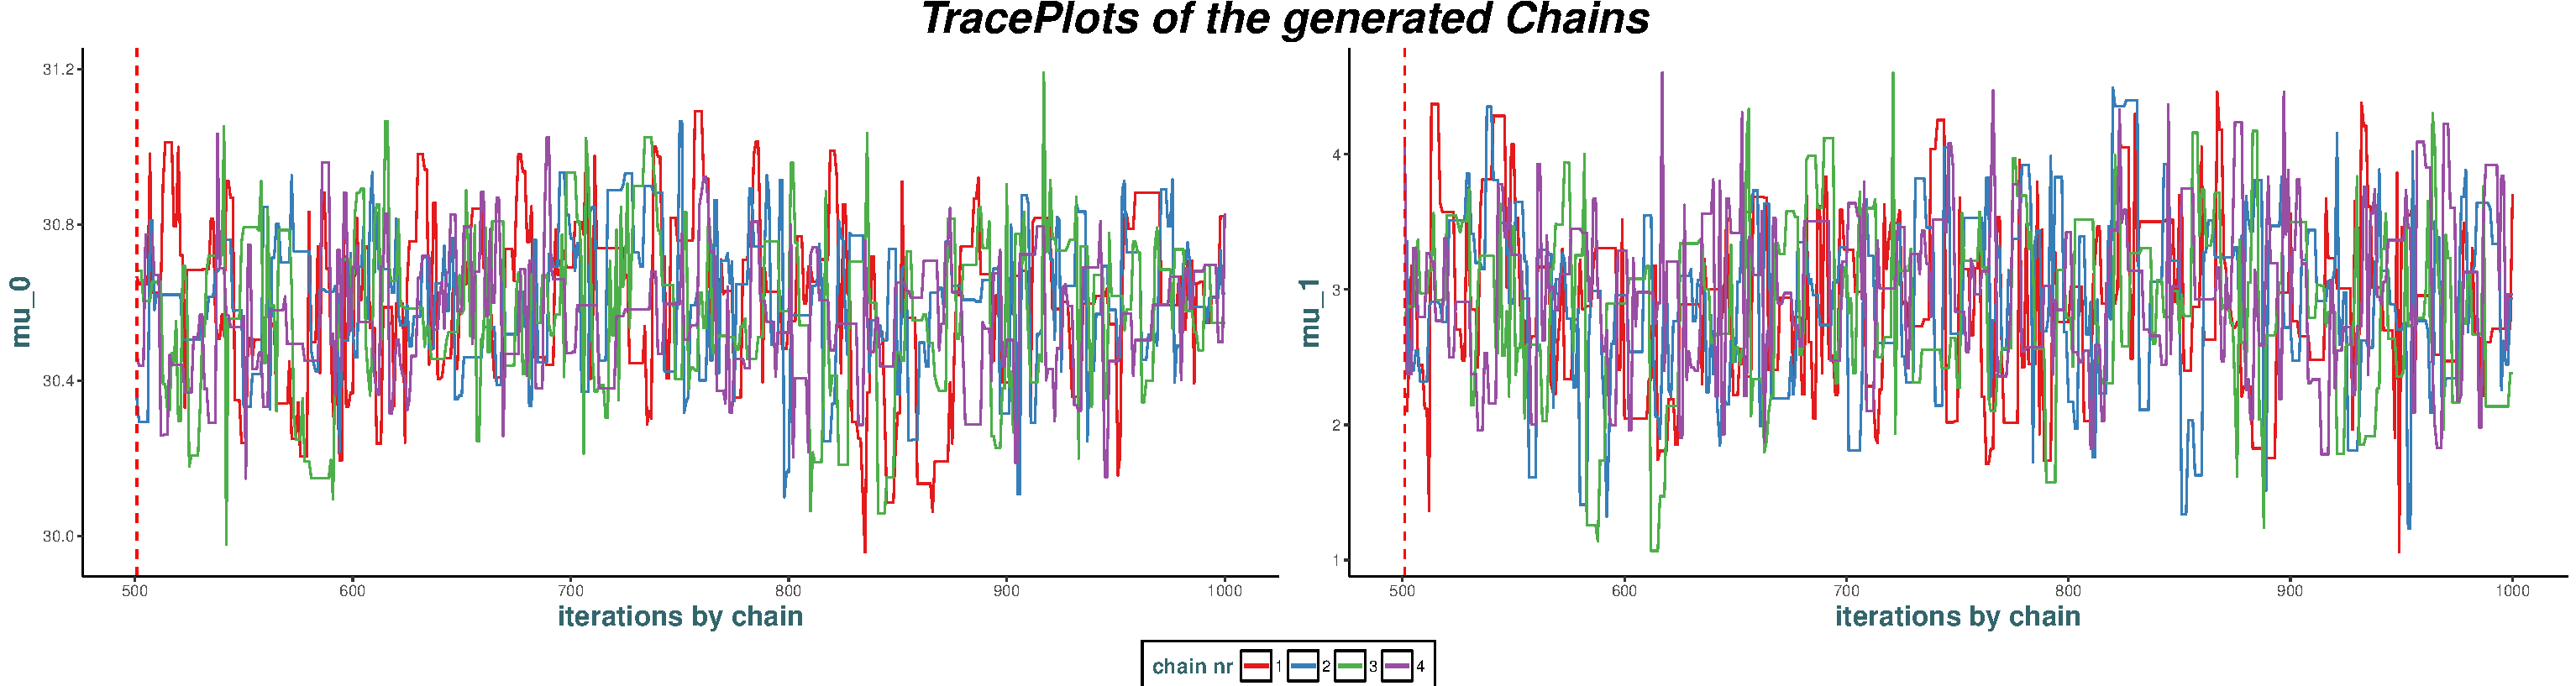
\includegraphics[width=1\linewidth]{chains1.pdf}
	\end{subfigure}
	
	\begin{subfigure}[b]{0.99\textwidth}
		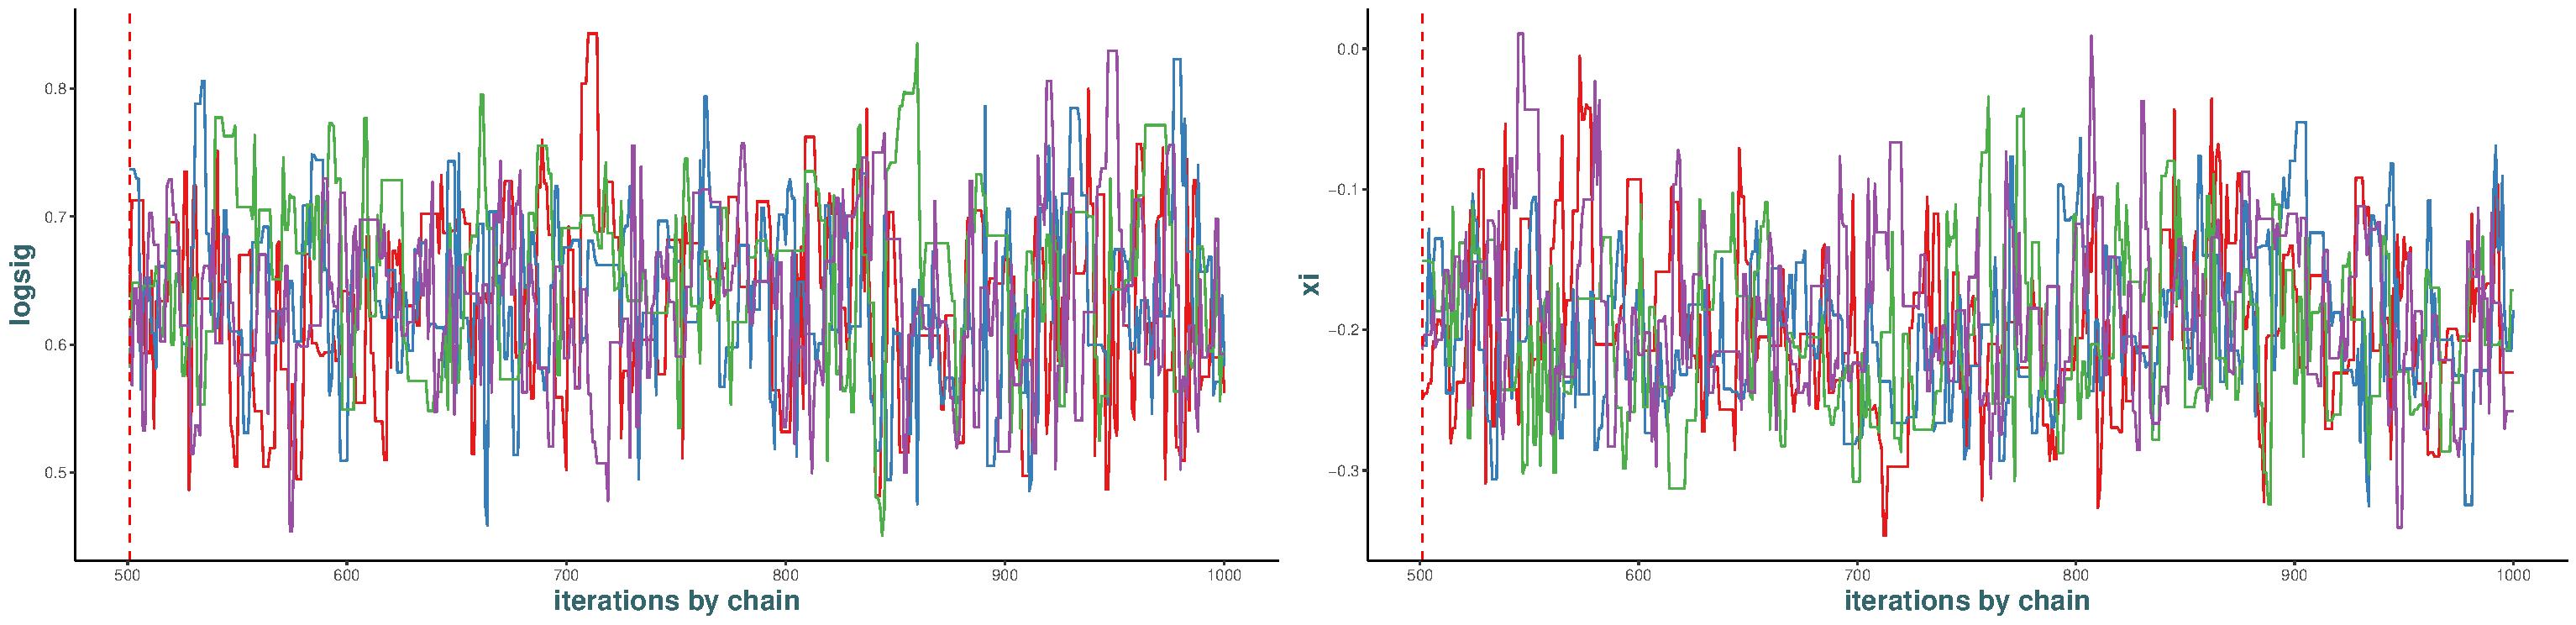
\includegraphics[width=1\linewidth]{chains2.pdf}
	\end{subfigure}
	\caption{Chains.. Note that the location parameter of the trend $\mu_1$ is of different order as in frequentist because we are absed on the rescaled values $t^*$ of $t$. We will transform it back for the inferences. }\label{fig:mixchains}
\end{figure}
Each parameter show chains that are mixing very well, reinforcing our confidence that the over-dispersed starting values we used have no influence on the target stationary distribution. 
We now gather all the chains with different starting values into a single chain, to obtain one single chain of size $N=2000$ for each parameter.


\subsubsection*{Gelman-Rubin}

The Gelman-Rubin diagnostic compares the behavior of the randomly initialized chains. It computes the $\hat{R}$ (\ref{eq:rhat}) or \emph{shrink factor} which measures the mixing of the chains. If convergence occurred, the $\hat{R}$ will be $1$.
The corresponding results are displayed in Figure \ref{fig:gelmdiag} in \hyperref[app:bayfig]{Appendix \textbf{\ref{app:bayfig}}}. It clearly shows that the parameter $\mu_0$ 
is 
As expected, it is a bit more tedious for the shape parameter, but it is especially tedious for $\log\sigma$ for which it takes at least $500$ iterations before $\hat{R}<1$. However, all parameters have $\hat{R}$ going very close to $1$ at the end of the iterations, showing thatour number of iterations $N$ should be sufficient..



\subsubsection*{Correlations within and between chains}


\begin{itemize}
	\item The \textbf{autocorrelations} of each parameter's Markov chain in Figure \ref{fig:autocor} in \hyperref[app:bayfig]{Appendix \textbf{\ref{app:bayfig}}} show are quickly decreasing with the lag. Again, it seems more problematic for $\log\sigma$ and $\xi$.	
	We have computed the effective sample size $N_{\text{eff}}$ from (\ref{eq:neff}), i.e. the sample size after correction for the autocorrelation in the chains :
	\begin{equation}
		N_{\text{eff}}^{(\mu_0)} = 389, \qquad 	N_{\text{eff}}^{(\mu_1)} = 436, \qquad 	N_{\text{eff}}^{(\nu)} = 194, \qquad	N_{\text{eff}}^{(\xi)} = 217.
	\end{equation}
	We can see the link of these values with the autocorrelations in Figure \ref{fig:autocor}.
	
	\item The \textbf{cross-correlation} in the parameters' Markov chains are depicted in Figure \ref{fig:crosscorr} in \hyperref[app:bayfig]{Appendix \textbf{\ref{app:bayfig}}}. We compared these values with the Fisher information matrix that we transformed in a correlation matrix, we found very similar values except for the correlation between the location parameters $\mu_0$ and $\mu_1$.
\end{itemize}


\subsubsection*{Geweke}

This diagnostic tests for the equality of the first $10\%$ of a chain with the mean computed from the second half of the chain. After the chain has been partitioned, the test is repeated $20$ times.
Figure \ref{fig:geweke} in \hyperref[app:bayfig]{Appendix \textbf{\ref{app:bayfig}}} shows the results. Quite surprisingly, $\mu_0$ has $6$ rejected values out of $20$, but these are really at the limit. Shape and log scale parameters are still somewhat problematic. However, we notice that this diagnostic is very diffuse.


\subsubsection*{Raftery and Lewis and Thinning}

One last diagnostic is from \citet{raftery1992} and provides interesting values on the chains, which are shown in Table \ref{tab:raf} in \hyperref[app:bayfig]{Appendix \textbf{\ref{app:bayfig}}}.

\begin{itemize} 
\item "$B$" is the avdised number of iterations to be discarded at the beginning of each chain.
\item "$N_{\text{advised}}$ " is the advised number of iterations.
\item "$N_{\text{min}}$ is the minimum sample size based on zero autocorrelation.
\item The "dependence factor" informs to which extent the autocorrelation in the chains inflates the required sample size, with values above 5 indicating a strong autocorrelation. 
\end{itemize}
Relatively high autocorrelations in the chains are again highlighted here.



\subsubsection*{Conclusion}

From the above results, i.e. the relatively high correlations within and between chains, it is recommended to increase the number of iterations $N$. Since the computational time is not huge, it it would be easily feasible, but in order to keep the same chains as presented above, we just decrease the burn-in period to $25\%$ to be left with $N=3000$. 


\subsection{Inference}\label{sec:bayinfci}

We present the results in Figure \ref{fig:postdens} with the Markov chains' Kernel posterior densities for each parameters, together with their $95\%$ Bayesian intervals. 

\begin{figure}[!htb]
	\centering	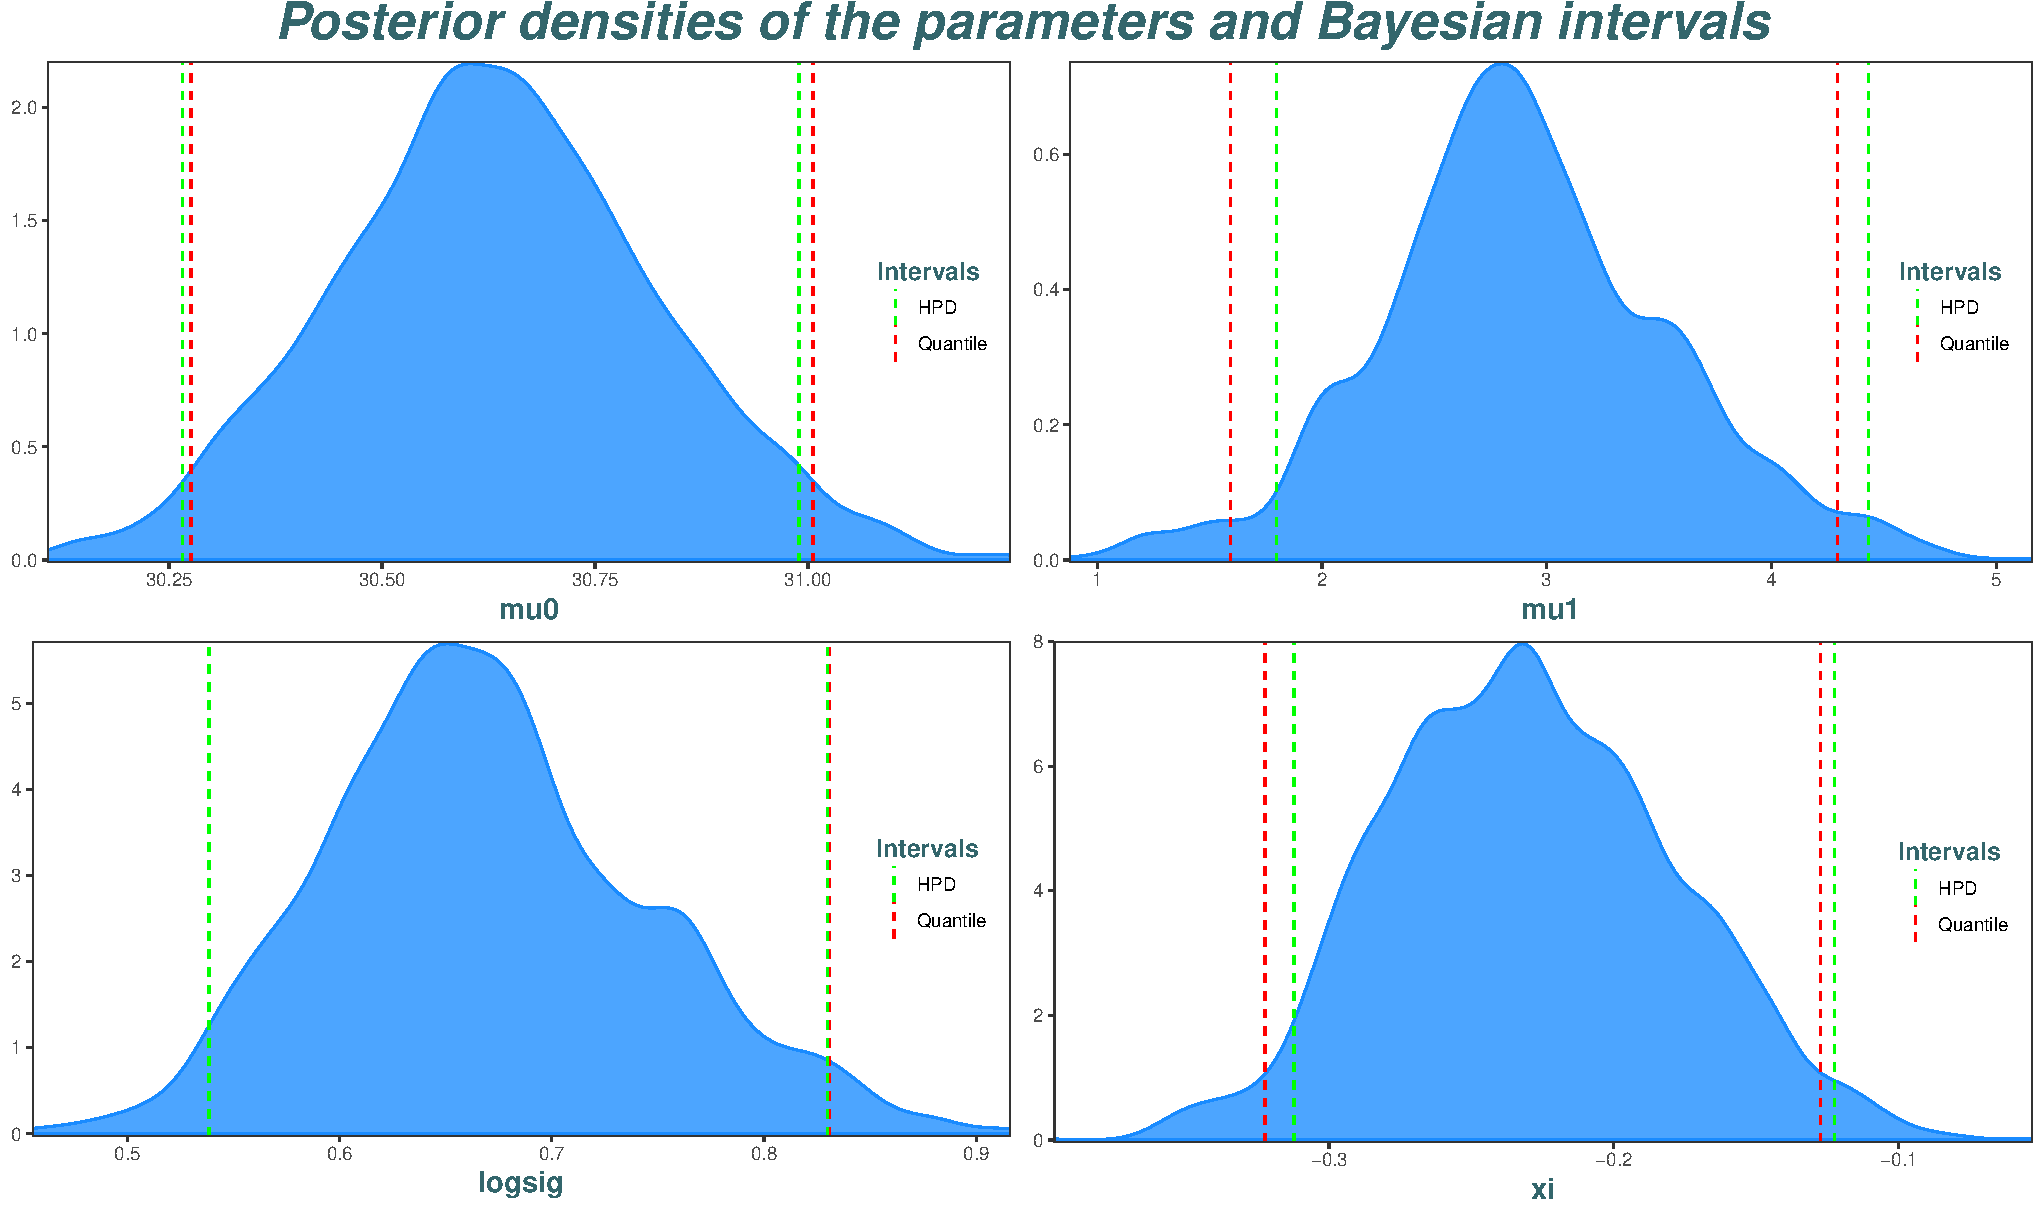
\includegraphics[width=0.8\linewidth]{postdens.pdf}\caption{Markov chains' Kernel posterior densities for the parameters. A Gaussian kernel with a bandwidth calculated by the \citet[pp.48, (3.31)]{silverman_1986} "rule of thumb" for each parameter has been used. Note that we did not make the back rescaling from $t^*$ to $t$, which explains the values of $\mu_1$.}\label{fig:postdens}
\end{figure}

We can see the differences between the two intervals when the densities are not symmetric. In this case, the highest-posterior density (HPD) intervals are slightly more precise.
These results are summarized in Table \ref{tab:postq} 

\begin{table}[!htbp] \centering 
	\caption{Table of quantiles of the posterior samples and of the posterior \textbf{mean}. We transformed back $\mu_1$ from $t^*$ to $t$ in years for comparisons with frequentist results. } \label{tab:postq} 
	\begin{tabular}{@{\extracolsep{5pt}} c|cccccc} 
\toprule
		& 2.5\% & 25\% & 50\% &  \textbf{mean} & 75\% & 97.5\% \\ 
\midrule
		$\mu_0$  & $30.276$ & $30.511$ & $30.632$ & $30.633$ & $30.754$ & $31.006$ \\ 
		$\mu_1$ & $0.0136$ & $0.0214$ & $0.0245$ & $0.0248$ & $0.0282$ & $0.0367$ \\ 
		$\log\sigma$ & $0.539$ & $0.617$ & $0.663$ &  $0.669$ &$0.717$ & $0.831$ \\ 
		$\xi$ & $-0.323$ & $-0.266$ & $-0.232$ & $-0.230$ & $-0.195$ & $-0.127$ \\ 
\bottomrule
		\end{tabular} 
\end{table} 
		

we see here that all the probability mass for the shape parameter is below $0$, i.e. $\Pr \Big\{\xi>0\Big\}=0$, reinforcing our confidence that we are under an EV-Weibull model. %without any doubts.

		
\subsection{Posterior Predictive Distribution} 

The Posterior Predictive Distribution (PPD) 

We expressely took $116$ years before as we know that it is not recommended to to make very long-term extrapolations. We first depict the results in Figure \ref{fig:ppd} where we represent the PPD with its $95\%$ credible intervals, together with the observed values from $1901$ to $2016$ and the values from $2016$ to $2131$ that have been simulated from the PPD.


 \begin{figure}[!htb]
 	\centering	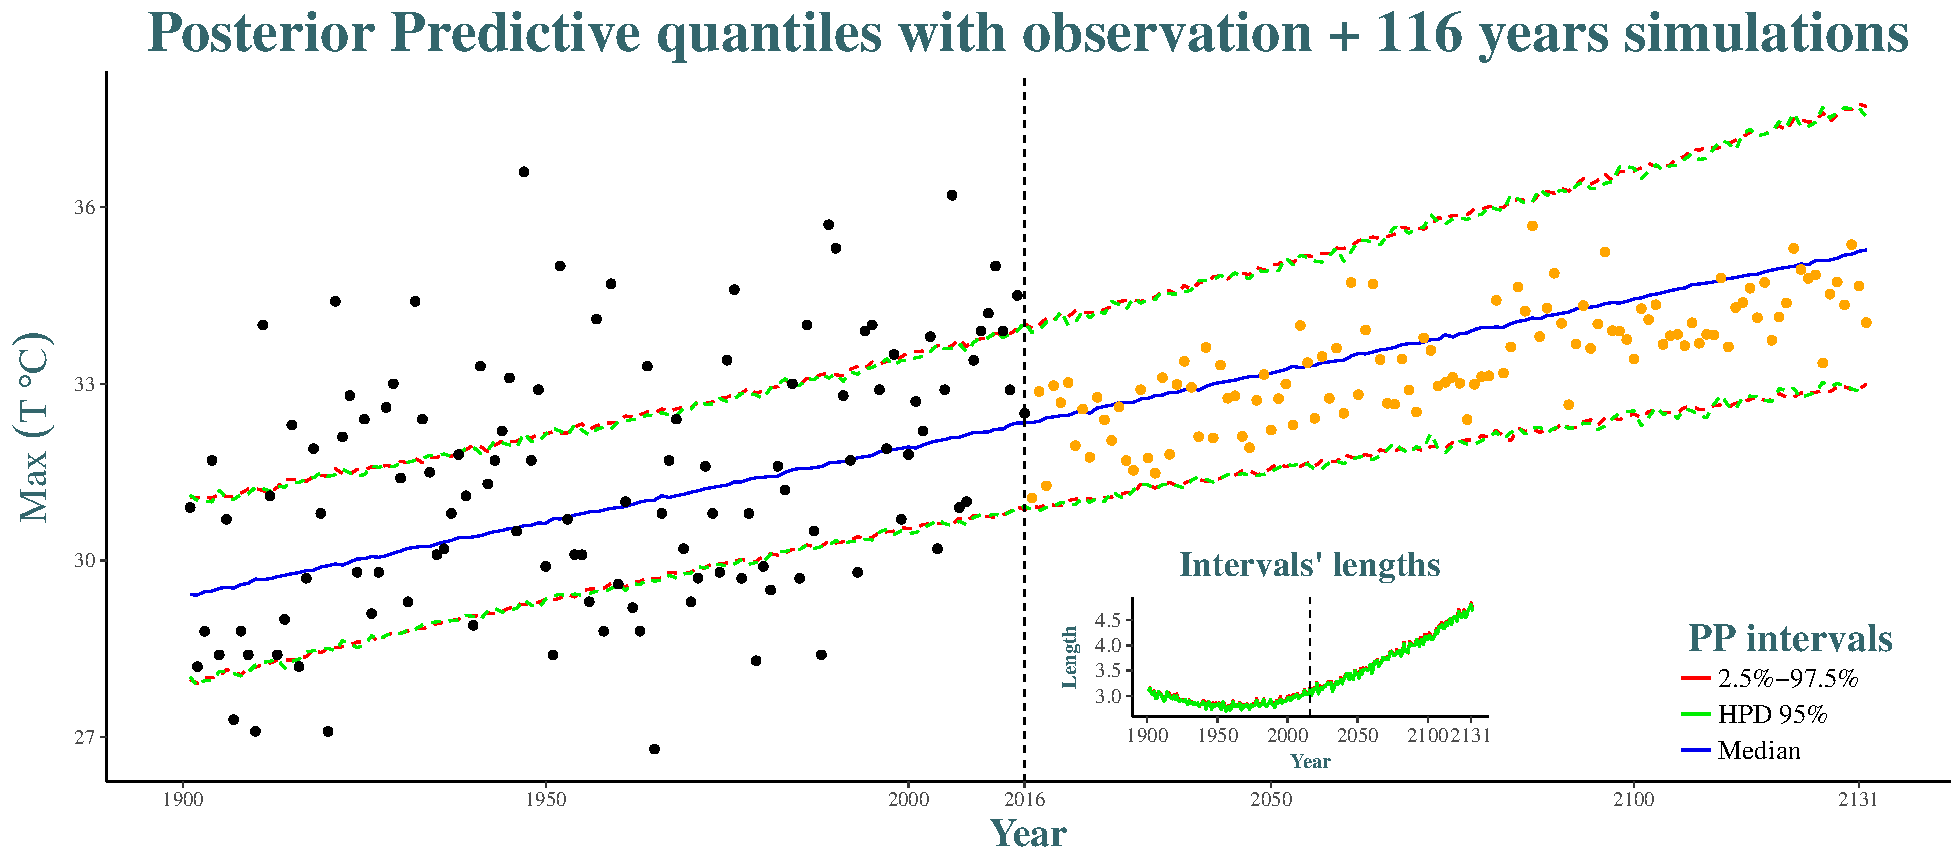
\includegraphics[width=0.9\linewidth]{ppd.pdf}\caption{Black dots represent the observations while orange dots represented the simulated values from the PPD. The printed plot aims to conveniently display the differences between the upper and the lower bounds of the two credible intervals considered.}\label{fig:ppd}
 \end{figure}
 
 This Figure \ref{fig:ppd} clearly highlights that the PP intervals are not $95\%$ credible intervals for the observed values but rather intervals for the posterior predicted values. Indeed, coverage analysis shows that the PP intervals cover $95\%$ of the simulated values from the PPD as the number of simulations becomes very high, but only $\approx 50\%$ for the observed values.
 
 
 The HPD and the quantile-based credible intervals are very similar here, for all the observations and simulations. 
 We can clearly visualize the Posterior Predictive credibility intervals having an increasing length  
 In fact, the evolution of the quantiles is linear in the range of data, and so is the PP median even beyond the range of the data. But, the 


 \begin{figure}[!htb]
  	\centering	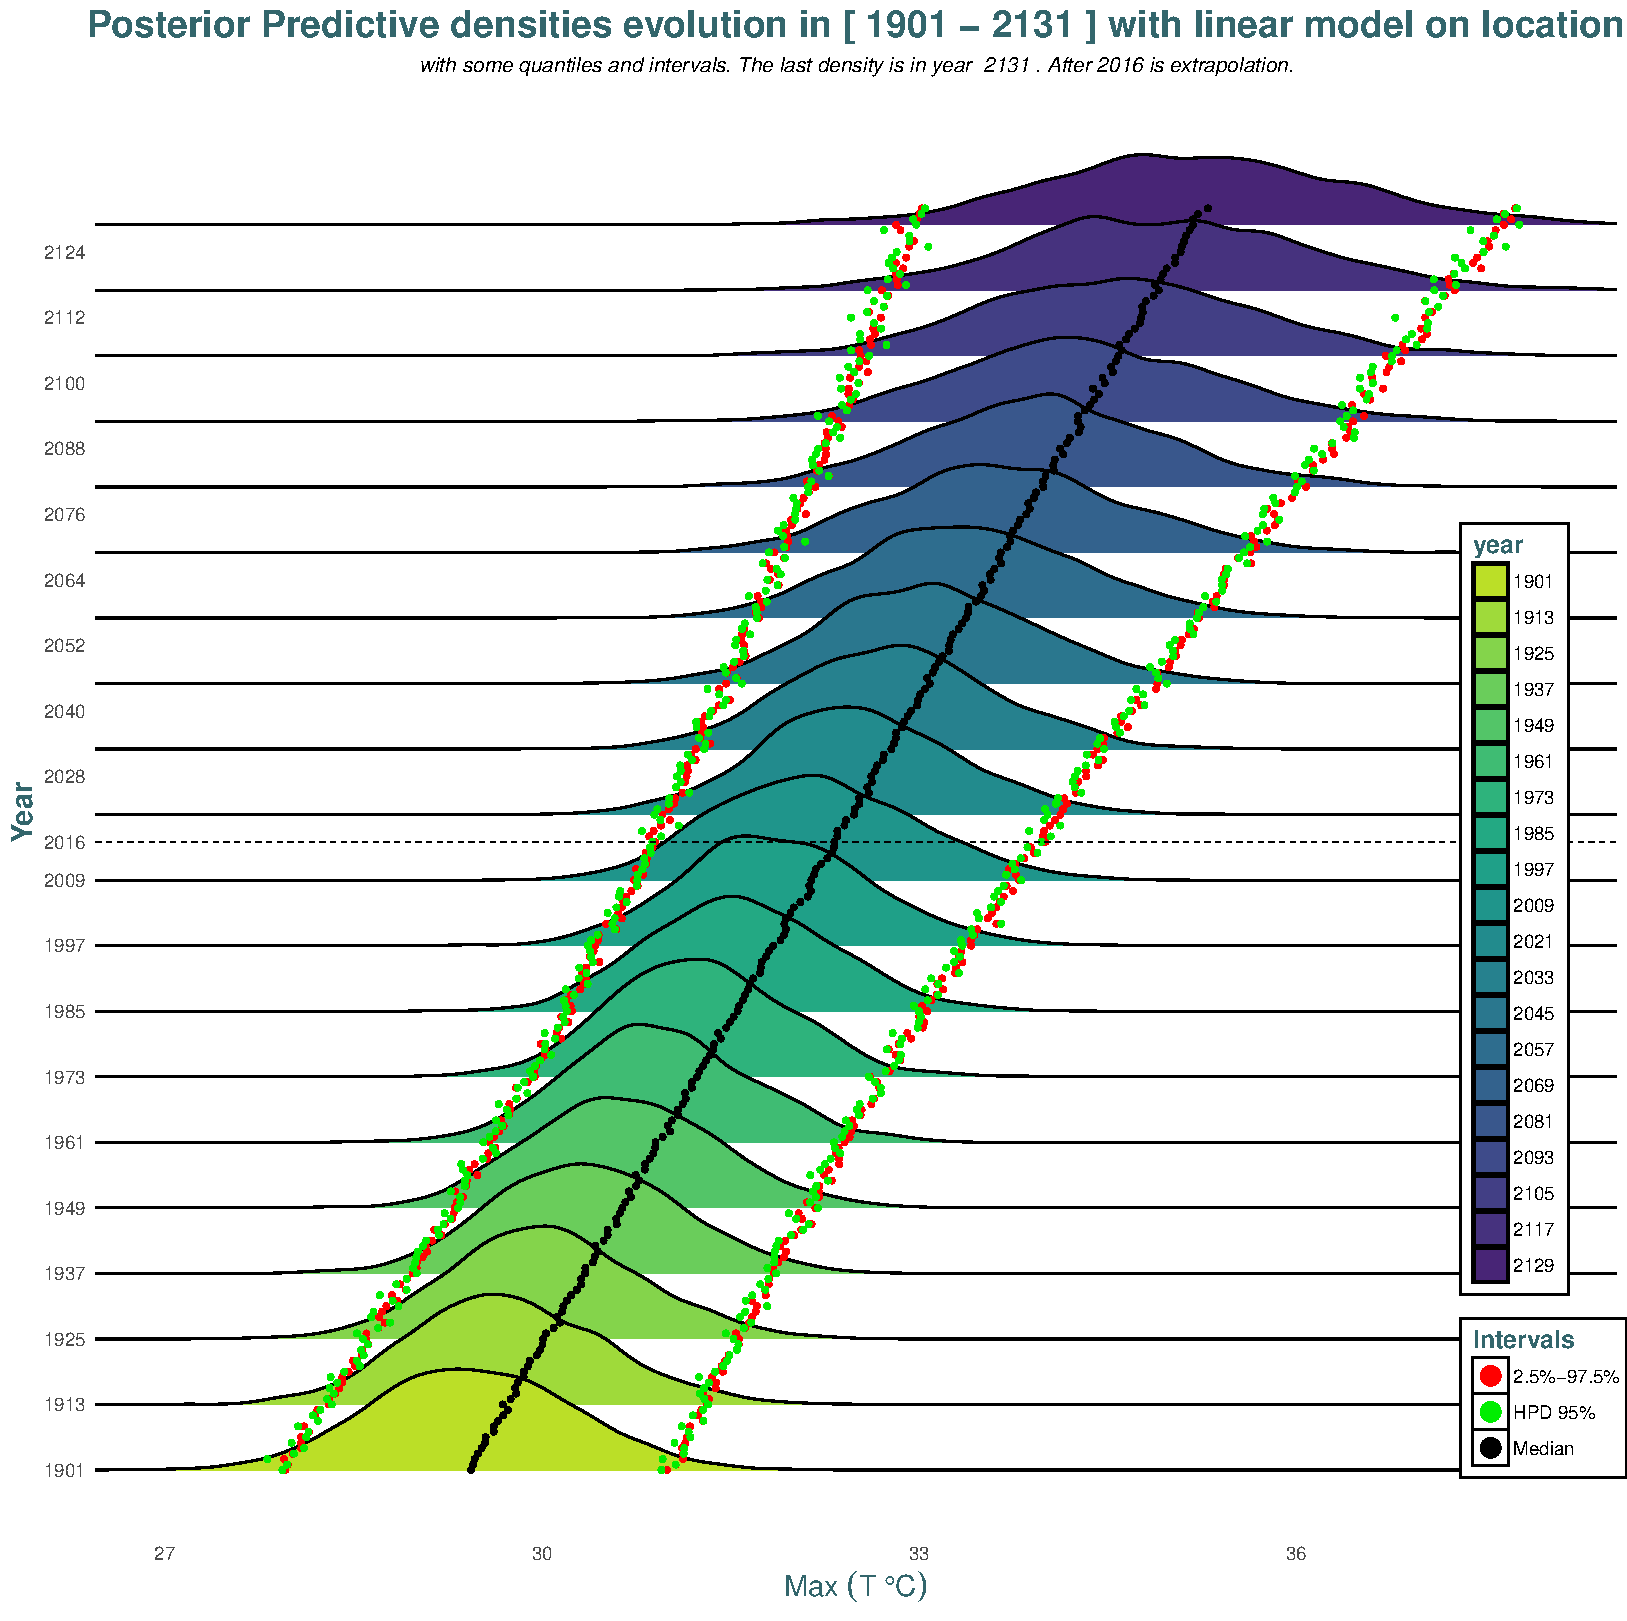
\includegraphics[width=0.8\linewidth]{predpred.pdf}\caption{A Gaussian kernel with a joint bandwidth calculated by the \citet[pp.48, (3.31)]{silverman_1986} "rule of thumb" is picked for each densities.}\label{fig:post_pred}
 \end{figure}
  
  We clearly see the linear trend with the temporal evolution of the quantiles...
  And the uncertainty from their deviation  from the median
  
  We remark from this graph the increasing variance of the predictive posterior as far as we predict in the future. It can also be seen from the $5\%$ and $95\%$ quantiles which deviate from the median. 
  
%\section{From HMC algorithm using STAN language}
%\section{Ratio of Uniform : \texttt{revdbayes} package}\label{sec:bayes_ratio}


\subsection{Return Levels}


We remind that quantiles of the fitted distribution can be more conveniently interpreted in EVT terminology as returns levels. Hence, the  Here, it is different since we are under the fitted PP distribution and not the fitted distribution. Indeed, these quantiles are taking the uncertainty of future prediction into account and are thus not strictly linearly increasing, while we have seen in Figure \ref{fig:rl_nsta} that the increase of the return levels was strictly linear even beyond the range of the data, although it was the same nonstationary model but in a frequentist setting. These are commonly called \emph{predictive return levels}. For example the above red line in Figure \ref{fig:ppd} is the $40$-year predictive return levels.

It is still also possible to compute the returns levels as in Figure \ref{fig:rl_nsta} by simply estimating the parameters (e.g. by their MC's posterior mean or median from Table \ref{tab:postq}). Then, the corresponding return levels can be computed relying on the values given to the parameters. Relying on the median, we verified that the return levels line is nearly the same for all points ; Bayesian return levels having a slightly higher intercept and slightly smaller slope compared to the line in Figure \ref{fig:rl_nsta}. 



\subsection{Sensitivity Analysis}

\textbf{section 7.4} evdbayes pdf + suppplément risk book 

"It is often the case that more than one model provides an adequate fit to the data. Sensitivity analysis determines by what extent posterior inferences change when alternative
models are used"   book risk analysis other section pp.2.



The basic sensitivity analysis works by fitting several models to
the same problem. Posterior inferences can then be compared.
The sensitivity of the
marginal posterior density of the shape parameter $\xi$ is often of particular interest.


The basic method of sensitivity analysis is to fit several models to the same problem.
 Posterior inferences from each model can then be compared. Posterior inferences
will typically include marginal posterior distributions of the 3 parameters posterior distributions of GEV quantiles and posterior predictive distributions.
The sensitivity of the marginal posterior density of the shape parameter $\xi$ is often of particular interest.



\section{Remarks and Comparison with Frequentist results}

In this first analysis, we rely on 



Comparing Table \ref{tab:postq} with Table 
 these look very similar. We must notice that is natural and this is rather comforting as we used non-informative priors so far. ( →→ study behaviour if we introduce information through priors ? )

The following Figure \ref{fig:cicomp} compares several intervals that have been computed during this thesis. 

\begin{itemize}
	\item The \emph{frequentist} confidence intervals computed in
	\hyperref[sec:xpstatio]{Section \textbf{\ref{sec:xpstatio}}}, comprising those coming from the normal approximation of the MLE and the profiled likelihood intervals.
	\item The \emph{bootstrap} confidence intervals computed in  \hyperref[sec:boot]{Section \textbf{\ref{sec:boot}}}, by the residual but also the parametric bootstrap. These intervals have not been computed for the location parameters since these were directly computed for $\mu(t)$ rather than $\mu_0$ and $\mu_1$. From the particular nature of these intervals which estimate parameters by GML and make use of prior distribution to compute the GEV-CDN weights, we will not consider these as truly "frequentist", but this is debatable.
	\item The \emph{Bayesian} credible intervals seen  above in \hyperref[sec:bayinfci]{Section \textbf{\ref{sec:bayinfci}}}.
\end{itemize}

\begin{figure}[!htb]
	\centering	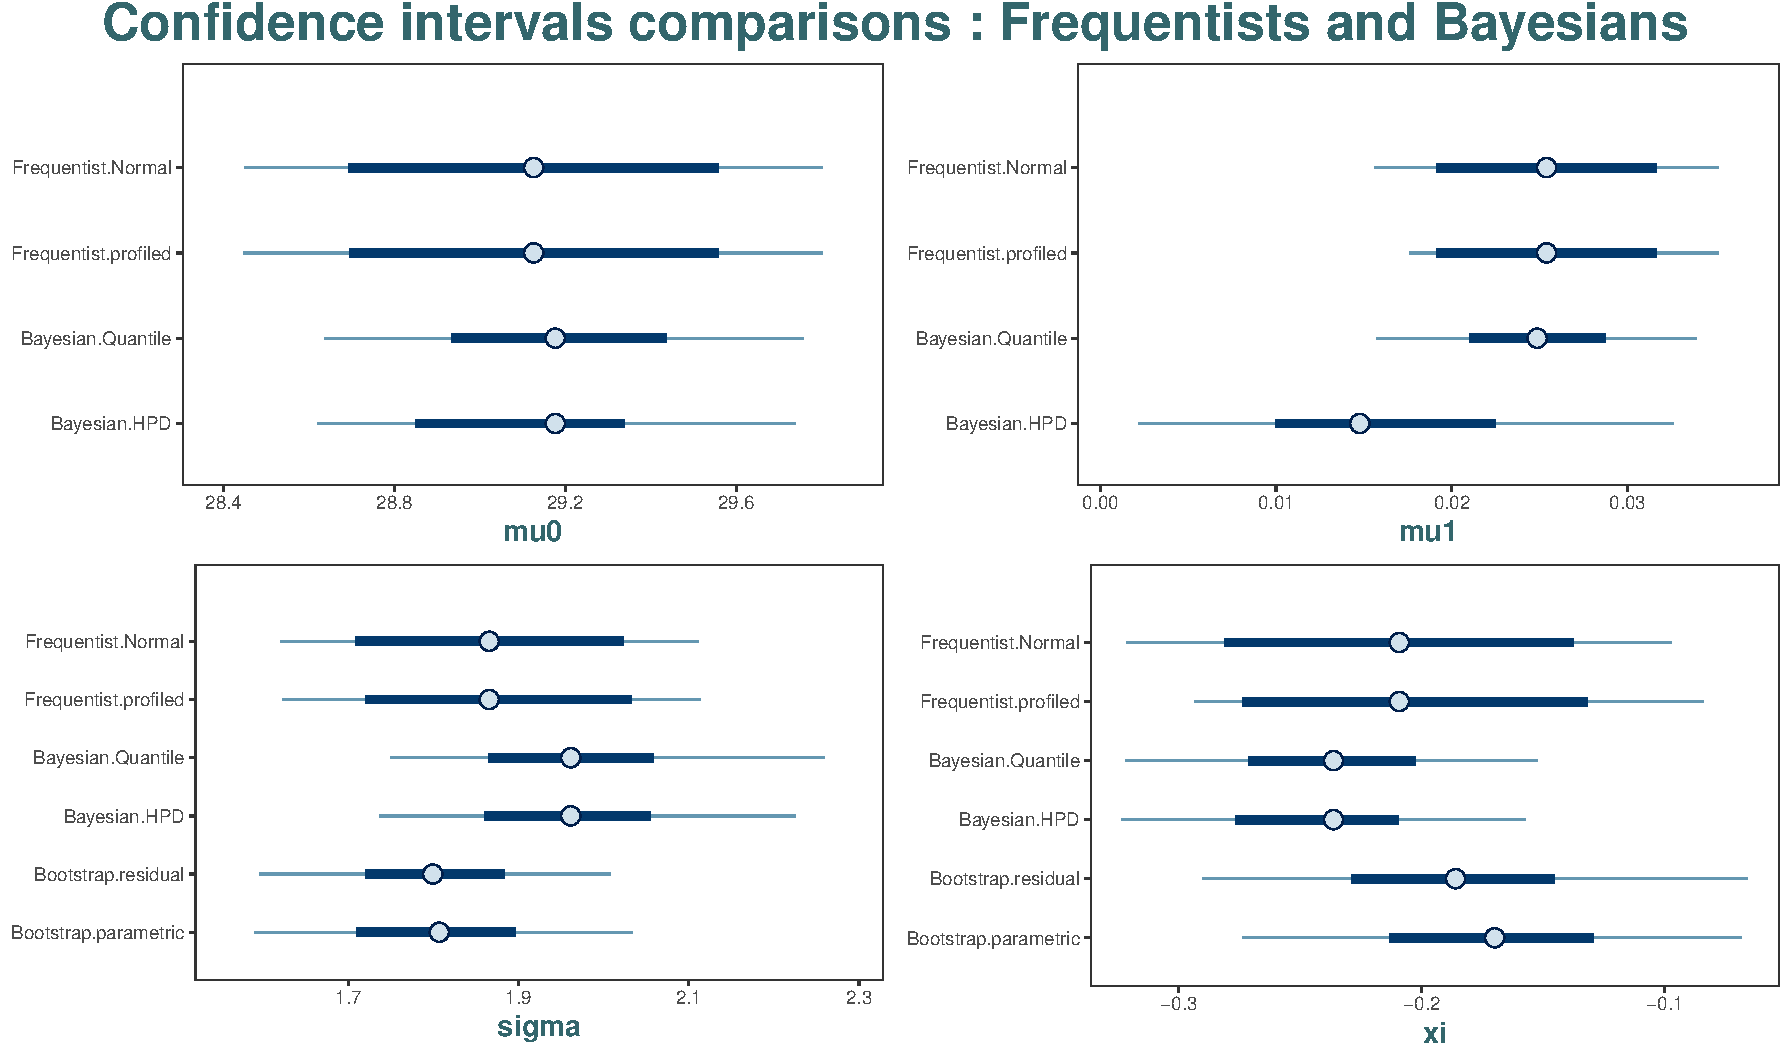
\includegraphics[width=0.9\linewidth]{cicomp.pdf}\caption{The center of the interval is the MLE for the frequentist intervals and the median for the Bayesian intervals. Thicker lines indicate $50\%$ confidence (or credibility) while thinner lines indicate $95\%$ intervals.}\label{fig:cicomp}
\end{figure}

The large differences between the Bayesian and the frequentist intervals for the parameter $\mu_0$ are due to 


By using objective priors (i.e. priors with very large variance), we should obtain the same results in the frequentist or in the Bayesian setting, which will be a prove of robustness of obtained results  

We could have used Bayesian model averaging, but


\subsubsection*{Discussion on the Prior used}

In all the analysis, we were not able to introduce knowledge through the specification of the prior. Hence, we will use non-informative priors (see \hyperref[sec:noninfoprior]{Section \textbf{\ref{sec:noninfoprior}}}), and in particular \emph{vague} (near-flat) independent normally distributed \emph{priors} (\ref{eq:vagprior}) for each parameter since this is the most convenient way to express our ignorance as showed by.


